\documentclass[twoside]{book}

% Packages required by doxygen
\usepackage{fixltx2e}
\usepackage{calc}
\usepackage{doxygen}
\usepackage[export]{adjustbox} % also loads graphicx
\usepackage{graphicx}
\usepackage[utf8]{inputenc}
\usepackage{makeidx}
\usepackage{multicol}
\usepackage{multirow}
\PassOptionsToPackage{warn}{textcomp}
\usepackage{textcomp}
\usepackage[nointegrals]{wasysym}
\usepackage[table]{xcolor}

% NLS support packages
\usepackage[spanish]{babel}
% Font selection
\usepackage[T1]{fontenc}
\usepackage[scaled=.90]{helvet}
\usepackage{courier}
\usepackage{amssymb}
\usepackage{sectsty}
\renewcommand{\familydefault}{\sfdefault}
\allsectionsfont{%
  \fontseries{bc}\selectfont%
  \color{darkgray}%
}
\renewcommand{\DoxyLabelFont}{%
  \fontseries{bc}\selectfont%
  \color{darkgray}%
}
\newcommand{\+}{\discretionary{\mbox{\scriptsize$\hookleftarrow$}}{}{}}

% Page & text layout
\usepackage{geometry}
\geometry{%
  a4paper,%
  top=2.5cm,%
  bottom=2.5cm,%
  left=2.5cm,%
  right=2.5cm%
}
\tolerance=750
\hfuzz=15pt
\hbadness=750
\setlength{\emergencystretch}{15pt}
\setlength{\parindent}{0cm}
\setlength{\parskip}{3ex plus 2ex minus 2ex}
\makeatletter
\renewcommand{\paragraph}{%
  \@startsection{paragraph}{4}{0ex}{-1.0ex}{1.0ex}{%
    \normalfont\normalsize\bfseries\SS@parafont%
  }%
}
\renewcommand{\subparagraph}{%
  \@startsection{subparagraph}{5}{0ex}{-1.0ex}{1.0ex}{%
    \normalfont\normalsize\bfseries\SS@subparafont%
  }%
}
\makeatother

% Headers & footers
\usepackage{fancyhdr}
\pagestyle{fancyplain}
\fancyhead[LE]{\fancyplain{}{\bfseries\thepage}}
\fancyhead[CE]{\fancyplain{}{}}
\fancyhead[RE]{\fancyplain{}{\bfseries\leftmark}}
\fancyhead[LO]{\fancyplain{}{\bfseries\rightmark}}
\fancyhead[CO]{\fancyplain{}{}}
\fancyhead[RO]{\fancyplain{}{\bfseries\thepage}}
\fancyfoot[LE]{\fancyplain{}{}}
\fancyfoot[CE]{\fancyplain{}{}}
\fancyfoot[RE]{\fancyplain{}{\bfseries\scriptsize Generado por Doxygen }}
\fancyfoot[LO]{\fancyplain{}{\bfseries\scriptsize Generado por Doxygen }}
\fancyfoot[CO]{\fancyplain{}{}}
\fancyfoot[RO]{\fancyplain{}{}}
\renewcommand{\footrulewidth}{0.4pt}
\renewcommand{\chaptermark}[1]{%
  \markboth{#1}{}%
}
\renewcommand{\sectionmark}[1]{%
  \markright{\thesection\ #1}%
}

% Indices & bibliography
\usepackage{natbib}
\usepackage[titles]{tocloft}
\setcounter{tocdepth}{3}
\setcounter{secnumdepth}{5}
\makeindex

% Hyperlinks (required, but should be loaded last)
\usepackage{ifpdf}
\ifpdf
  \usepackage[pdftex,pagebackref=true]{hyperref}
\else
  \usepackage[ps2pdf,pagebackref=true]{hyperref}
\fi
\hypersetup{%
  colorlinks=true,%
  linkcolor=blue,%
  citecolor=blue,%
  unicode%
}

% Custom commands
\newcommand{\clearemptydoublepage}{%
  \newpage{\pagestyle{empty}\cleardoublepage}%
}

\usepackage{caption}
\captionsetup{labelsep=space,justification=centering,font={bf},singlelinecheck=off,skip=4pt,position=top}

%===== C O N T E N T S =====

\begin{document}

% Titlepage & ToC
\hypersetup{pageanchor=false,
             bookmarksnumbered=true,
             pdfencoding=unicode
            }
\pagenumbering{roman}
\begin{titlepage}
\vspace*{7cm}
\begin{center}%
{\Large P1 }\\
\vspace*{1cm}
{\large Generado por Doxygen 1.8.11}\\
\end{center}
\end{titlepage}
\clearemptydoublepage
\tableofcontents
\clearemptydoublepage
\pagenumbering{arabic}
\hypersetup{pageanchor=true}

%--- Begin generated contents ---
\chapter{Indice de archivos}
\section{Lista de archivos}
Lista de todos los archivos documentados y con descripciones breves\+:\begin{DoxyCompactList}
\item\contentsline{section}{\hyperlink{ejercicio10_8c}{ejercicio10.\+c} \\*Implementa el ejercicio 10 de mascaras }{\pageref{ejercicio10_8c}}{}
\item\contentsline{section}{\hyperlink{ejercicio3a_8c}{ejercicio3a.\+c} \\*Implementa el ejercicio 3a de procesos con un solo padre }{\pageref{ejercicio3a_8c}}{}
\item\contentsline{section}{\hyperlink{ejercicio3b_8c}{ejercicio3b.\+c} \\*Implementa el ejercicio 3b de hilos de un proceso }{\pageref{ejercicio3b_8c}}{}
\item\contentsline{section}{\hyperlink{ejercicio4a_8c}{ejercicio4a.\+c} \\*Implementa el ejercicio 4a de multiplicacion de matrices }{\pageref{ejercicio4a_8c}}{}
\item\contentsline{section}{\hyperlink{ejercicio4b_8c}{ejercicio4b.\+c} \\*Implementa el ejercicio 4b de multiplicacion de matrices }{\pageref{ejercicio4b_8c}}{}
\item\contentsline{section}{\hyperlink{ejercicio6_8c}{ejercicio6.\+c} \\*Implementa el ejercicio 6 de señales }{\pageref{ejercicio6_8c}}{}
\end{DoxyCompactList}

\chapter{Documentación de archivos}
\hypertarget{ejercicio4ai_8c}{}\section{Referencia del Archivo ejercicio4ai.\+c}
\label{ejercicio4ai_8c}\index{ejercicio4ai.\+c@{ejercicio4ai.\+c}}


Implementa el ejercicio 4a pedido para analizar su arbol de procesos.  


{\ttfamily \#include $<$stdio.\+h$>$}\\*
{\ttfamily \#include $<$stdlib.\+h$>$}\\*
{\ttfamily \#include $<$sys/types.\+h$>$}\\*
{\ttfamily \#include $<$sys/wait.\+h$>$}\\*
{\ttfamily \#include $<$unistd.\+h$>$}\\*
Dependencia gráfica adjunta para ejercicio4ai.\+c\+:
\nopagebreak
\begin{figure}[H]
\begin{center}
\leavevmode
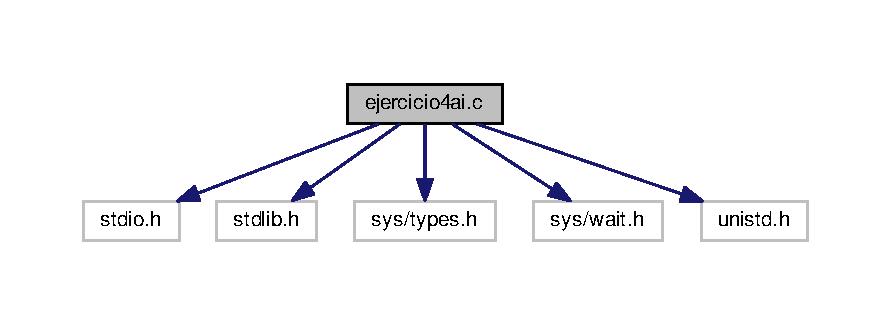
\includegraphics[width=350pt]{ejercicio4ai_8c__incl}
\end{center}
\end{figure}
\subsection*{\textquotesingle{}defines\textquotesingle{}}
\begin{DoxyCompactItemize}
\item 
\#define \hyperlink{ejercicio4ai_8c_acee2369f62e4a096d243dec3cd7d0b00}{N\+U\+M\+\_\+\+P\+R\+OC}~3
\end{DoxyCompactItemize}
\subsection*{Funciones}
\begin{DoxyCompactItemize}
\item 
int \hyperlink{ejercicio4ai_8c_a840291bc02cba5474a4cb46a9b9566fe}{main} (void)
\begin{DoxyCompactList}\small\item\em funcion dada para ser analizada \end{DoxyCompactList}\end{DoxyCompactItemize}


\subsection{Descripción detallada}
Implementa el ejercicio 4a pedido para analizar su arbol de procesos. 

\begin{DoxyAuthor}{Autor}
Andres Salas \href{mailto:andres.salas@estudiante.uam.es}{\tt andres.\+salas@estudiante.\+uam.\+es} 

Antonio Martin \href{mailto:antonio.martinmasuda@estudiante.uam.es}{\tt antonio.\+martinmasuda@estudiante.\+uam.\+es} 
\end{DoxyAuthor}
\begin{DoxyNote}{Nota}
Grupo 2202 
\end{DoxyNote}
\begin{DoxyVersion}{Versión}
I) Copia del codigo dado para analizar su arbol 
\end{DoxyVersion}
\begin{DoxyDate}{Fecha}
03/02/2017 
\end{DoxyDate}


\subsection{Documentación de los \textquotesingle{}defines\textquotesingle{}}
\index{ejercicio4ai.\+c@{ejercicio4ai.\+c}!N\+U\+M\+\_\+\+P\+R\+OC@{N\+U\+M\+\_\+\+P\+R\+OC}}
\index{N\+U\+M\+\_\+\+P\+R\+OC@{N\+U\+M\+\_\+\+P\+R\+OC}!ejercicio4ai.\+c@{ejercicio4ai.\+c}}
\subsubsection[{\texorpdfstring{N\+U\+M\+\_\+\+P\+R\+OC}{NUM_PROC}}]{\setlength{\rightskip}{0pt plus 5cm}\#define N\+U\+M\+\_\+\+P\+R\+OC~3}\hypertarget{ejercicio4ai_8c_acee2369f62e4a096d243dec3cd7d0b00}{}\label{ejercicio4ai_8c_acee2369f62e4a096d243dec3cd7d0b00}
Numero de procesos del bucle for dado 

\subsection{Documentación de las funciones}
\index{ejercicio4ai.\+c@{ejercicio4ai.\+c}!main@{main}}
\index{main@{main}!ejercicio4ai.\+c@{ejercicio4ai.\+c}}
\subsubsection[{\texorpdfstring{main(void)}{main(void)}}]{\setlength{\rightskip}{0pt plus 5cm}int main (
\begin{DoxyParamCaption}
\item[{void}]{}
\end{DoxyParamCaption}
)}\hypertarget{ejercicio4ai_8c_a840291bc02cba5474a4cb46a9b9566fe}{}\label{ejercicio4ai_8c_a840291bc02cba5474a4cb46a9b9566fe}


funcion dada para ser analizada 

\begin{DoxyReturn}{Devuelve}
int\+: valor de exito o fracaso 
\end{DoxyReturn}

\hypertarget{ejercicio4aii_8c}{}\section{Referencia del Archivo ejercicio4aii.\+c}
\label{ejercicio4aii_8c}\index{ejercicio4aii.\+c@{ejercicio4aii.\+c}}


Implementa el ejercicio 4a con los cambios pedidos.  


{\ttfamily \#include $<$stdio.\+h$>$}\\*
{\ttfamily \#include $<$stdlib.\+h$>$}\\*
{\ttfamily \#include $<$sys/types.\+h$>$}\\*
{\ttfamily \#include $<$sys/wait.\+h$>$}\\*
{\ttfamily \#include $<$unistd.\+h$>$}\\*
Dependencia gráfica adjunta para ejercicio4aii.\+c\+:
\nopagebreak
\begin{figure}[H]
\begin{center}
\leavevmode
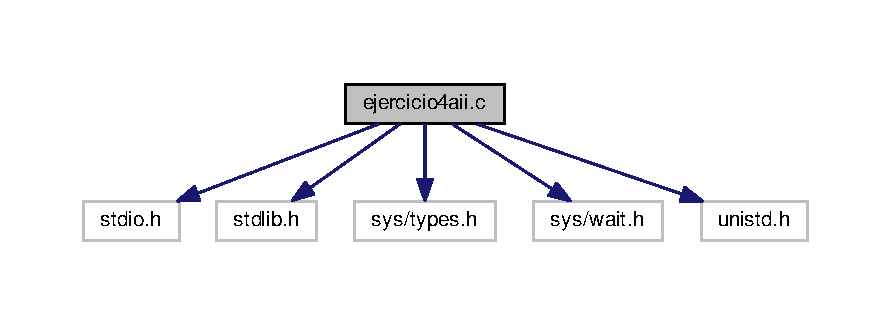
\includegraphics[width=350pt]{ejercicio4aii_8c__incl}
\end{center}
\end{figure}
\subsection*{\textquotesingle{}defines\textquotesingle{}}
\begin{DoxyCompactItemize}
\item 
\#define \hyperlink{ejercicio4aii_8c_acee2369f62e4a096d243dec3cd7d0b00}{N\+U\+M\+\_\+\+P\+R\+OC}~3
\end{DoxyCompactItemize}
\subsection*{Funciones}
\begin{DoxyCompactItemize}
\item 
int \hyperlink{ejercicio4aii_8c_a840291bc02cba5474a4cb46a9b9566fe}{main} (void)
\begin{DoxyCompactList}\small\item\em funcion en la que el hijo imprime su pid y el del padre \end{DoxyCompactList}\end{DoxyCompactItemize}


\subsection{Descripción detallada}
Implementa el ejercicio 4a con los cambios pedidos. 

\begin{DoxyAuthor}{Autor}
Andres Salas \href{mailto:andres.salas@estudiante.uam.es}{\tt andres.\+salas@estudiante.\+uam.\+es} 

Antonio Martin \href{mailto:antonio.martinmasuda@estudiante.uam.es}{\tt antonio.\+martinmasuda@estudiante.\+uam.\+es} 
\end{DoxyAuthor}
\begin{DoxyNote}{Nota}
Grupo 2202 
\end{DoxyNote}
\begin{DoxyVersion}{Versión}
II) Cambios en el codigo dado. 
\end{DoxyVersion}
\begin{DoxyDate}{Fecha}
03/02/2017 
\end{DoxyDate}


\subsection{Documentación de los \textquotesingle{}defines\textquotesingle{}}
\index{ejercicio4aii.\+c@{ejercicio4aii.\+c}!N\+U\+M\+\_\+\+P\+R\+OC@{N\+U\+M\+\_\+\+P\+R\+OC}}
\index{N\+U\+M\+\_\+\+P\+R\+OC@{N\+U\+M\+\_\+\+P\+R\+OC}!ejercicio4aii.\+c@{ejercicio4aii.\+c}}
\subsubsection[{\texorpdfstring{N\+U\+M\+\_\+\+P\+R\+OC}{NUM_PROC}}]{\setlength{\rightskip}{0pt plus 5cm}\#define N\+U\+M\+\_\+\+P\+R\+OC~3}\hypertarget{ejercicio4aii_8c_acee2369f62e4a096d243dec3cd7d0b00}{}\label{ejercicio4aii_8c_acee2369f62e4a096d243dec3cd7d0b00}
Numero de procesos del bucle for dado 

\subsection{Documentación de las funciones}
\index{ejercicio4aii.\+c@{ejercicio4aii.\+c}!main@{main}}
\index{main@{main}!ejercicio4aii.\+c@{ejercicio4aii.\+c}}
\subsubsection[{\texorpdfstring{main(void)}{main(void)}}]{\setlength{\rightskip}{0pt plus 5cm}int main (
\begin{DoxyParamCaption}
\item[{void}]{}
\end{DoxyParamCaption}
)}\hypertarget{ejercicio4aii_8c_a840291bc02cba5474a4cb46a9b9566fe}{}\label{ejercicio4aii_8c_a840291bc02cba5474a4cb46a9b9566fe}


funcion en la que el hijo imprime su pid y el del padre 

\begin{DoxyReturn}{Devuelve}
int\+: valor de exito o fracaso 
\end{DoxyReturn}

\hypertarget{ejercicio4bi_8c}{}\section{Referencia del Archivo ejercicio4bi.\+c}
\label{ejercicio4bi_8c}\index{ejercicio4bi.\+c@{ejercicio4bi.\+c}}


Implementa el ejercicio 4b pedido para analizar sus diferencias con a)  


{\ttfamily \#include $<$stdio.\+h$>$}\\*
{\ttfamily \#include $<$stdlib.\+h$>$}\\*
{\ttfamily \#include $<$sys/types.\+h$>$}\\*
{\ttfamily \#include $<$sys/wait.\+h$>$}\\*
{\ttfamily \#include $<$unistd.\+h$>$}\\*
Dependencia gráfica adjunta para ejercicio4bi.\+c\+:
\nopagebreak
\begin{figure}[H]
\begin{center}
\leavevmode
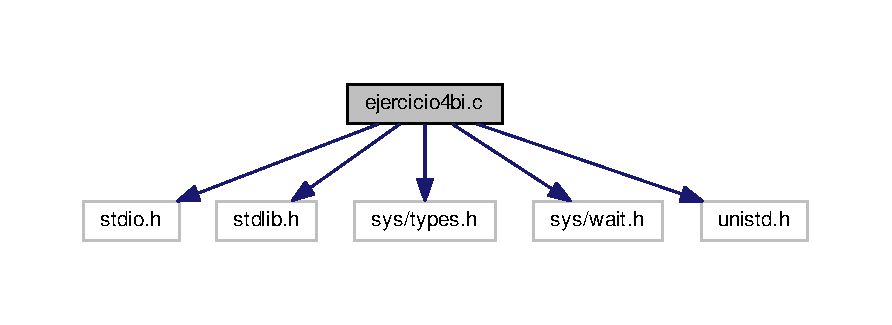
\includegraphics[width=350pt]{ejercicio4bi_8c__incl}
\end{center}
\end{figure}
\subsection*{\textquotesingle{}defines\textquotesingle{}}
\begin{DoxyCompactItemize}
\item 
\#define \hyperlink{ejercicio4bi_8c_acee2369f62e4a096d243dec3cd7d0b00}{N\+U\+M\+\_\+\+P\+R\+OC}~3
\end{DoxyCompactItemize}
\subsection*{Funciones}
\begin{DoxyCompactItemize}
\item 
int \hyperlink{ejercicio4bi_8c_a840291bc02cba5474a4cb46a9b9566fe}{main} (void)
\begin{DoxyCompactList}\small\item\em funcion dada para ser analizada \end{DoxyCompactList}\end{DoxyCompactItemize}


\subsection{Descripción detallada}
Implementa el ejercicio 4b pedido para analizar sus diferencias con a) 

\begin{DoxyAuthor}{Autor}
Andres Salas \href{mailto:andres.salas@estudiante.uam.es}{\tt andres.\+salas@estudiante.\+uam.\+es} 

Antonio Martin \href{mailto:antonio.martinmasuda@estudiante.uam.es}{\tt antonio.\+martinmasuda@estudiante.\+uam.\+es} 
\end{DoxyAuthor}
\begin{DoxyNote}{Nota}
Grupo 2202 
\end{DoxyNote}
\begin{DoxyVersion}{Versión}
I) Copia del codigo dado para analizar sus diferencias con a) 
\end{DoxyVersion}
\begin{DoxyDate}{Fecha}
03/02/2017 
\end{DoxyDate}


\subsection{Documentación de los \textquotesingle{}defines\textquotesingle{}}
\index{ejercicio4bi.\+c@{ejercicio4bi.\+c}!N\+U\+M\+\_\+\+P\+R\+OC@{N\+U\+M\+\_\+\+P\+R\+OC}}
\index{N\+U\+M\+\_\+\+P\+R\+OC@{N\+U\+M\+\_\+\+P\+R\+OC}!ejercicio4bi.\+c@{ejercicio4bi.\+c}}
\subsubsection[{\texorpdfstring{N\+U\+M\+\_\+\+P\+R\+OC}{NUM_PROC}}]{\setlength{\rightskip}{0pt plus 5cm}\#define N\+U\+M\+\_\+\+P\+R\+OC~3}\hypertarget{ejercicio4bi_8c_acee2369f62e4a096d243dec3cd7d0b00}{}\label{ejercicio4bi_8c_acee2369f62e4a096d243dec3cd7d0b00}
Numero de procesos del bucle for dado 

\subsection{Documentación de las funciones}
\index{ejercicio4bi.\+c@{ejercicio4bi.\+c}!main@{main}}
\index{main@{main}!ejercicio4bi.\+c@{ejercicio4bi.\+c}}
\subsubsection[{\texorpdfstring{main(void)}{main(void)}}]{\setlength{\rightskip}{0pt plus 5cm}int main (
\begin{DoxyParamCaption}
\item[{void}]{}
\end{DoxyParamCaption}
)}\hypertarget{ejercicio4bi_8c_a840291bc02cba5474a4cb46a9b9566fe}{}\label{ejercicio4bi_8c_a840291bc02cba5474a4cb46a9b9566fe}


funcion dada para ser analizada 

\begin{DoxyReturn}{Devuelve}
int\+: valor de exito o fracaso 
\end{DoxyReturn}

\hypertarget{ejercicio4bii_8c}{}\section{Referencia del Archivo ejercicio4bii.\+c}
\label{ejercicio4bii_8c}\index{ejercicio4bii.\+c@{ejercicio4bii.\+c}}


Implementa el ejercicio 4b con los cambios pedidos.  


{\ttfamily \#include $<$stdio.\+h$>$}\\*
{\ttfamily \#include $<$stdlib.\+h$>$}\\*
{\ttfamily \#include $<$sys/types.\+h$>$}\\*
{\ttfamily \#include $<$sys/wait.\+h$>$}\\*
{\ttfamily \#include $<$unistd.\+h$>$}\\*
Dependencia gráfica adjunta para ejercicio4bii.\+c\+:
\nopagebreak
\begin{figure}[H]
\begin{center}
\leavevmode
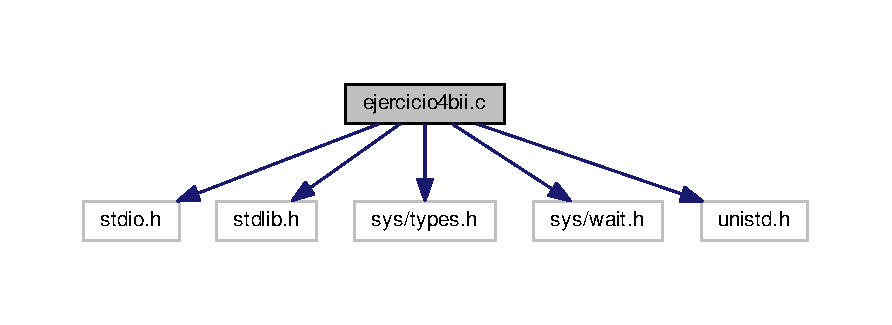
\includegraphics[width=350pt]{ejercicio4bii_8c__incl}
\end{center}
\end{figure}
\subsection*{\textquotesingle{}defines\textquotesingle{}}
\begin{DoxyCompactItemize}
\item 
\#define \hyperlink{ejercicio4bii_8c_acee2369f62e4a096d243dec3cd7d0b00}{N\+U\+M\+\_\+\+P\+R\+OC}~3
\end{DoxyCompactItemize}
\subsection*{Funciones}
\begin{DoxyCompactItemize}
\item 
int \hyperlink{ejercicio4bii_8c_a840291bc02cba5474a4cb46a9b9566fe}{main} (void)
\begin{DoxyCompactList}\small\item\em funcion en la que el hijo imprime su pid y el del padre \end{DoxyCompactList}\end{DoxyCompactItemize}


\subsection{Descripción detallada}
Implementa el ejercicio 4b con los cambios pedidos. 

\begin{DoxyAuthor}{Autor}
Andres Salas \href{mailto:andres.salas@estudiante.uam.es}{\tt andres.\+salas@estudiante.\+uam.\+es} 

Antonio Martin \href{mailto:antonio.martinmasuda@estudiante.uam.es}{\tt antonio.\+martinmasuda@estudiante.\+uam.\+es} 
\end{DoxyAuthor}
\begin{DoxyNote}{Nota}
Grupo 2202 
\end{DoxyNote}
\begin{DoxyVersion}{Versión}
II) Cambios en el codigo dado. 
\end{DoxyVersion}
\begin{DoxyDate}{Fecha}
03/02/2017 
\end{DoxyDate}


\subsection{Documentación de los \textquotesingle{}defines\textquotesingle{}}
\index{ejercicio4bii.\+c@{ejercicio4bii.\+c}!N\+U\+M\+\_\+\+P\+R\+OC@{N\+U\+M\+\_\+\+P\+R\+OC}}
\index{N\+U\+M\+\_\+\+P\+R\+OC@{N\+U\+M\+\_\+\+P\+R\+OC}!ejercicio4bii.\+c@{ejercicio4bii.\+c}}
\subsubsection[{\texorpdfstring{N\+U\+M\+\_\+\+P\+R\+OC}{NUM_PROC}}]{\setlength{\rightskip}{0pt plus 5cm}\#define N\+U\+M\+\_\+\+P\+R\+OC~3}\hypertarget{ejercicio4bii_8c_acee2369f62e4a096d243dec3cd7d0b00}{}\label{ejercicio4bii_8c_acee2369f62e4a096d243dec3cd7d0b00}
Numero de procesos del bucle for dado 

\subsection{Documentación de las funciones}
\index{ejercicio4bii.\+c@{ejercicio4bii.\+c}!main@{main}}
\index{main@{main}!ejercicio4bii.\+c@{ejercicio4bii.\+c}}
\subsubsection[{\texorpdfstring{main(void)}{main(void)}}]{\setlength{\rightskip}{0pt plus 5cm}int main (
\begin{DoxyParamCaption}
\item[{void}]{}
\end{DoxyParamCaption}
)}\hypertarget{ejercicio4bii_8c_a840291bc02cba5474a4cb46a9b9566fe}{}\label{ejercicio4bii_8c_a840291bc02cba5474a4cb46a9b9566fe}


funcion en la que el hijo imprime su pid y el del padre 

\begin{DoxyReturn}{Devuelve}
int\+: valor de exito o fracaso 
\end{DoxyReturn}

\hypertarget{ejercicio5a_8c}{}\section{Referencia del Archivo ejercicio5a.\+c}
\label{ejercicio5a_8c}\index{ejercicio5a.\+c@{ejercicio5a.\+c}}


Implementa el ejercicio 5a de procesos secuenciales.  


{\ttfamily \#include $<$stdio.\+h$>$}\\*
{\ttfamily \#include $<$stdlib.\+h$>$}\\*
{\ttfamily \#include $<$sys/types.\+h$>$}\\*
{\ttfamily \#include $<$sys/wait.\+h$>$}\\*
{\ttfamily \#include $<$unistd.\+h$>$}\\*
Dependencia gráfica adjunta para ejercicio5a.\+c\+:\nopagebreak
\begin{figure}[H]
\begin{center}
\leavevmode
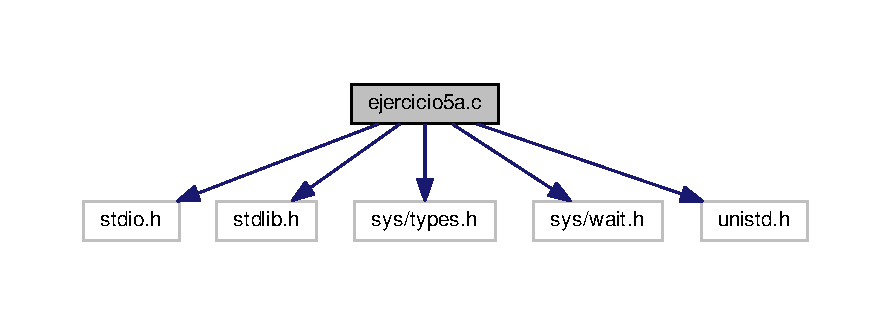
\includegraphics[width=350pt]{ejercicio5a_8c__incl}
\end{center}
\end{figure}
\subsection*{\textquotesingle{}defines\textquotesingle{}}
\begin{DoxyCompactItemize}
\item 
\#define \hyperlink{ejercicio5a_8c_acee2369f62e4a096d243dec3cd7d0b00}{N\+U\+M\+\_\+\+P\+R\+OC}~3
\end{DoxyCompactItemize}
\subsection*{Funciones}
\begin{DoxyCompactItemize}
\item 
int \hyperlink{ejercicio5a_8c_a840291bc02cba5474a4cb46a9b9566fe}{main} (void)
\begin{DoxyCompactList}\small\item\em funcion de procesos secuenciales \end{DoxyCompactList}\end{DoxyCompactItemize}


\subsection{Descripción detallada}
Implementa el ejercicio 5a de procesos secuenciales. 

\begin{DoxyAuthor}{Autor}
Andres Salas \href{mailto:andres.salas@estudiante.uam.es}{\tt andres.\+salas@estudiante.\+uam.\+es} 

Antonio Martin \href{mailto:antonio.martinmasuda@estudiante.uam.es}{\tt antonio.\+martinmasuda@estudiante.\+uam.\+es} 
\end{DoxyAuthor}
\begin{DoxyNote}{Nota}
Grupo 2202 
\end{DoxyNote}
\begin{DoxyVersion}{Versión}
1.\+0 
\end{DoxyVersion}
\begin{DoxyDate}{Fecha}
10/02/2017 
\end{DoxyDate}


\subsection{Documentación de los \textquotesingle{}defines\textquotesingle{}}
\index{ejercicio5a.\+c@{ejercicio5a.\+c}!N\+U\+M\+\_\+\+P\+R\+OC@{N\+U\+M\+\_\+\+P\+R\+OC}}
\index{N\+U\+M\+\_\+\+P\+R\+OC@{N\+U\+M\+\_\+\+P\+R\+OC}!ejercicio5a.\+c@{ejercicio5a.\+c}}
\subsubsection[{\texorpdfstring{N\+U\+M\+\_\+\+P\+R\+OC}{NUM_PROC}}]{\setlength{\rightskip}{0pt plus 5cm}\#define N\+U\+M\+\_\+\+P\+R\+OC~3}\hypertarget{ejercicio5a_8c_acee2369f62e4a096d243dec3cd7d0b00}{}\label{ejercicio5a_8c_acee2369f62e4a096d243dec3cd7d0b00}
Numero de procesos del bucle for dado 

\subsection{Documentación de las funciones}
\index{ejercicio5a.\+c@{ejercicio5a.\+c}!main@{main}}
\index{main@{main}!ejercicio5a.\+c@{ejercicio5a.\+c}}
\subsubsection[{\texorpdfstring{main(void)}{main(void)}}]{\setlength{\rightskip}{0pt plus 5cm}int main (
\begin{DoxyParamCaption}
\item[{void}]{}
\end{DoxyParamCaption}
)}\hypertarget{ejercicio5a_8c_a840291bc02cba5474a4cb46a9b9566fe}{}\label{ejercicio5a_8c_a840291bc02cba5474a4cb46a9b9566fe}


funcion de procesos secuenciales 

\begin{DoxyReturn}{Devuelve}
int\+: valor de exito o fracaso 
\end{DoxyReturn}

\hypertarget{ejercicio5b_8c}{}\section{Referencia del Archivo ejercicio5b.\+c}
\label{ejercicio5b_8c}\index{ejercicio5b.\+c@{ejercicio5b.\+c}}


Implementa el ejercicio 5b de semaforos (test con N-\/\+A\+R\+I\+OS)  


{\ttfamily \#include \char`\"{}semaforos.\+h\char`\"{}}\\*
{\ttfamily \#include $<$sys/sem.\+h$>$}\\*
Dependencia gráfica adjunta para ejercicio5b.\+c\+:\nopagebreak
\begin{figure}[H]
\begin{center}
\leavevmode
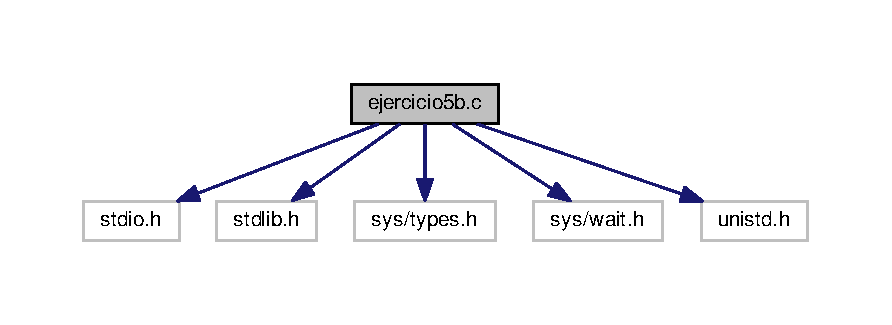
\includegraphics[width=251pt]{ejercicio5b_8c__incl}
\end{center}
\end{figure}
\subsection*{\textquotesingle{}defines\textquotesingle{}}
\begin{DoxyCompactItemize}
\item 
\#define \hyperlink{ejercicio5b_8c_ada831b9e37399bf906c8184a888e28cd}{S\+E\+M\+K\+EY}~75798\hypertarget{ejercicio5b_8c_ada831b9e37399bf906c8184a888e28cd}{}\label{ejercicio5b_8c_ada831b9e37399bf906c8184a888e28cd}

\begin{DoxyCompactList}\small\item\em Define la clave precompartida de los semaforos. \end{DoxyCompactList}\item 
\#define \hyperlink{ejercicio5b_8c_a95c81905ff3d55e62fb763f407f9fab1}{N\+\_\+\+S\+E\+M\+A\+F\+O\+R\+OS}~3\hypertarget{ejercicio5b_8c_a95c81905ff3d55e62fb763f407f9fab1}{}\label{ejercicio5b_8c_a95c81905ff3d55e62fb763f407f9fab1}

\begin{DoxyCompactList}\small\item\em Define el numero total de semaforos. \end{DoxyCompactList}\end{DoxyCompactItemize}
\subsection*{Funciones}
\begin{DoxyCompactItemize}
\item 
int \hyperlink{ejercicio5b_8c_ae66f6b31b5ad750f1fe042a706a4e3d4}{main} ()
\begin{DoxyCompactList}\small\item\em funcion principal/ test con semaforos B\+I\+N\+A\+R\+I\+OS y N-\/\+A\+R\+I\+OS siguiendo el codigo se explica que se va realizando \end{DoxyCompactList}\end{DoxyCompactItemize}


\subsection{Descripción detallada}
Implementa el ejercicio 5b de semaforos (test con N-\/\+A\+R\+I\+OS) 

\begin{DoxyAuthor}{Autor}
Andres Salas \href{mailto:andres.salas@estudiante.uam.es}{\tt andres.\+salas@estudiante.\+uam.\+es} 

Antonio Martin \href{mailto:antonio.martinmasuda@estudiante.uam.es}{\tt antonio.\+martinmasuda@estudiante.\+uam.\+es} 
\end{DoxyAuthor}
\begin{DoxyNote}{Nota}
Grupo 2202 
\end{DoxyNote}
\begin{DoxyVersion}{Versión}
1.\+0 
\end{DoxyVersion}
\begin{DoxyDate}{Fecha}
05/03/2017 
\end{DoxyDate}


\subsection{Documentación de las funciones}
\index{ejercicio5b.\+c@{ejercicio5b.\+c}!main@{main}}
\index{main@{main}!ejercicio5b.\+c@{ejercicio5b.\+c}}
\subsubsection[{\texorpdfstring{main()}{main()}}]{\setlength{\rightskip}{0pt plus 5cm}int main (
\begin{DoxyParamCaption}
{}
\end{DoxyParamCaption}
)}\hypertarget{ejercicio5b_8c_ae66f6b31b5ad750f1fe042a706a4e3d4}{}\label{ejercicio5b_8c_ae66f6b31b5ad750f1fe042a706a4e3d4}


funcion principal/ test con semaforos B\+I\+N\+A\+R\+I\+OS y N-\/\+A\+R\+I\+OS siguiendo el codigo se explica que se va realizando 

\begin{DoxyReturn}{Devuelve}
int\+: valor de exito (OK) o fracaso (E\+R\+R\+OR) 
\end{DoxyReturn}

\hypertarget{ejercicio6_8c}{}\section{Referencia del Archivo ejercicio6.\+c}
\label{ejercicio6_8c}\index{ejercicio6.\+c@{ejercicio6.\+c}}


Implementa el ejercicio 6 de relacion entre procesos padre/hijo.  


{\ttfamily \#include $<$stdio.\+h$>$}\\*
{\ttfamily \#include $<$stdlib.\+h$>$}\\*
{\ttfamily \#include $<$sys/types.\+h$>$}\\*
{\ttfamily \#include $<$sys/wait.\+h$>$}\\*
{\ttfamily \#include $<$unistd.\+h$>$}\\*
Dependencia gráfica adjunta para ejercicio6.\+c\+:\nopagebreak
\begin{figure}[H]
\begin{center}
\leavevmode
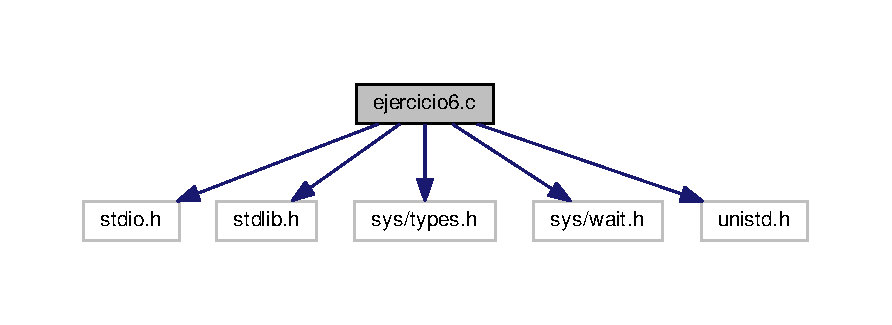
\includegraphics[width=350pt]{ejercicio6_8c__incl}
\end{center}
\end{figure}
\subsection*{\textquotesingle{}defines\textquotesingle{}}
\begin{DoxyCompactItemize}
\item 
\#define \hyperlink{ejercicio6_8c_a4cc8fa399feaab01926e82767a97a96b}{C\+A\+D\+E\+NA}~80
\end{DoxyCompactItemize}
\subsection*{Funciones}
\begin{DoxyCompactItemize}
\item 
int \hyperlink{ejercicio6_8c_a840291bc02cba5474a4cb46a9b9566fe}{main} (void)
\begin{DoxyCompactList}\small\item\em funcion en la que el proceso padre reserva memoria y en el proceso hijo el usuario introduce un nombre \end{DoxyCompactList}\end{DoxyCompactItemize}


\subsection{Descripción detallada}
Implementa el ejercicio 6 de relacion entre procesos padre/hijo. 

\begin{DoxyAuthor}{Autor}
Andres Salas \href{mailto:andres.salas@estudiante.uam.es}{\tt andres.\+salas@estudiante.\+uam.\+es} 

Antonio Martin \href{mailto:antonio.martinmasuda@estudiante.uam.es}{\tt antonio.\+martinmasuda@estudiante.\+uam.\+es} 
\end{DoxyAuthor}
\begin{DoxyNote}{Nota}
Grupo 2202 
\end{DoxyNote}
\begin{DoxyVersion}{Versión}
1.\+0 
\end{DoxyVersion}
\begin{DoxyDate}{Fecha}
10/02/2017 
\end{DoxyDate}


\subsection{Documentación de los \textquotesingle{}defines\textquotesingle{}}
\index{ejercicio6.\+c@{ejercicio6.\+c}!C\+A\+D\+E\+NA@{C\+A\+D\+E\+NA}}
\index{C\+A\+D\+E\+NA@{C\+A\+D\+E\+NA}!ejercicio6.\+c@{ejercicio6.\+c}}
\subsubsection[{\texorpdfstring{C\+A\+D\+E\+NA}{CADENA}}]{\setlength{\rightskip}{0pt plus 5cm}\#define C\+A\+D\+E\+NA~80}\hypertarget{ejercicio6_8c_a4cc8fa399feaab01926e82767a97a96b}{}\label{ejercicio6_8c_a4cc8fa399feaab01926e82767a97a96b}
Numero de caracteres de la cadena 

\subsection{Documentación de las funciones}
\index{ejercicio6.\+c@{ejercicio6.\+c}!main@{main}}
\index{main@{main}!ejercicio6.\+c@{ejercicio6.\+c}}
\subsubsection[{\texorpdfstring{main(void)}{main(void)}}]{\setlength{\rightskip}{0pt plus 5cm}int main (
\begin{DoxyParamCaption}
\item[{void}]{}
\end{DoxyParamCaption}
)}\hypertarget{ejercicio6_8c_a840291bc02cba5474a4cb46a9b9566fe}{}\label{ejercicio6_8c_a840291bc02cba5474a4cb46a9b9566fe}


funcion en la que el proceso padre reserva memoria y en el proceso hijo el usuario introduce un nombre 

\begin{DoxyReturn}{Devuelve}
int\+: valor de exito o fracaso 
\end{DoxyReturn}

\hypertarget{ejercicio8_8c}{}\section{Referencia del Archivo ejercicio8.\+c}
\label{ejercicio8_8c}\index{ejercicio8.\+c@{ejercicio8.\+c}}


Implementa el ejercicio 8 de ejecucion.  


{\ttfamily \#include $<$stdio.\+h$>$}\\*
{\ttfamily \#include $<$stdlib.\+h$>$}\\*
{\ttfamily \#include $<$string.\+h$>$}\\*
{\ttfamily \#include $<$unistd.\+h$>$}\\*
{\ttfamily \#include $<$sys/types.\+h$>$}\\*
{\ttfamily \#include $<$sys/wait.\+h$>$}\\*
Dependencia gráfica adjunta para ejercicio8.\+c\+:
\nopagebreak
\begin{figure}[H]
\begin{center}
\leavevmode
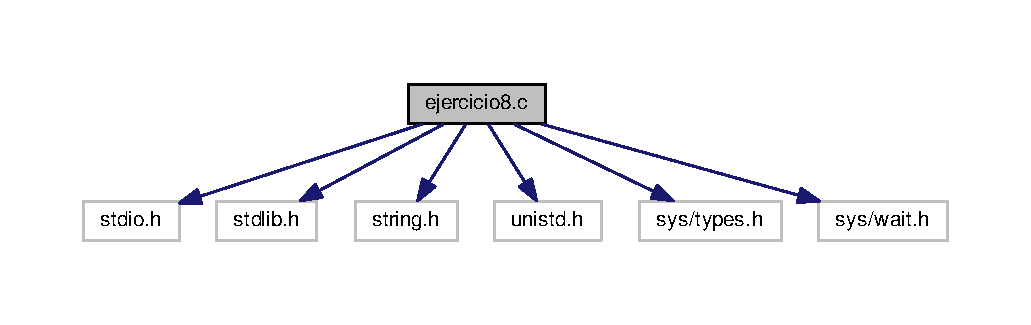
\includegraphics[width=350pt]{ejercicio8_8c__incl}
\end{center}
\end{figure}
\subsection*{Funciones}
\begin{DoxyCompactItemize}
\item 
char $\ast$ {\bfseries get\+Programa} (char $\ast$path)\hypertarget{ejercicio8_8c_a26bcb1e99a7cfca86a1e63abed7c5bbb}{}\label{ejercicio8_8c_a26bcb1e99a7cfca86a1e63abed7c5bbb}

\item 
int {\bfseries main} (int argc, char $\ast$argv\mbox{[}$\,$\mbox{]})\hypertarget{ejercicio8_8c_a0ddf1224851353fc92bfbff6f499fa97}{}\label{ejercicio8_8c_a0ddf1224851353fc92bfbff6f499fa97}

\end{DoxyCompactItemize}


\subsection{Descripción detallada}
Implementa el ejercicio 8 de ejecucion. 

\begin{DoxyAuthor}{Autor}
Andres Salas \href{mailto:andres.salas@estudiante.uam.es}{\tt andres.\+salas@estudiante.\+uam.\+es} 

Antonio Martin \href{mailto:antonio.martinmasuda@estudiante.uam.es}{\tt antonio.\+martinmasuda@estudiante.\+uam.\+es} 
\end{DoxyAuthor}
\begin{DoxyNote}{Nota}
Grupo 2202 
\end{DoxyNote}
\begin{DoxyVersion}{Versión}
1.\+0 
\end{DoxyVersion}
\begin{DoxyDate}{Fecha}
17/02/2017 
\end{DoxyDate}

\hypertarget{ejercicio9_8c}{}\section{Referencia del Archivo ejercicio9.\+c}
\label{ejercicio9_8c}\index{ejercicio9.\+c@{ejercicio9.\+c}}


Implementa el ejercicio 9 de tuberias.  


{\ttfamily \#include $<$stdio.\+h$>$}\\*
{\ttfamily \#include $<$stdlib.\+h$>$}\\*
{\ttfamily \#include $<$string.\+h$>$}\\*
{\ttfamily \#include $<$sys/types.\+h$>$}\\*
{\ttfamily \#include $<$sys/wait.\+h$>$}\\*
{\ttfamily \#include $<$unistd.\+h$>$}\\*
Dependencia gráfica adjunta para ejercicio9.\+c\+:
\nopagebreak
\begin{figure}[H]
\begin{center}
\leavevmode
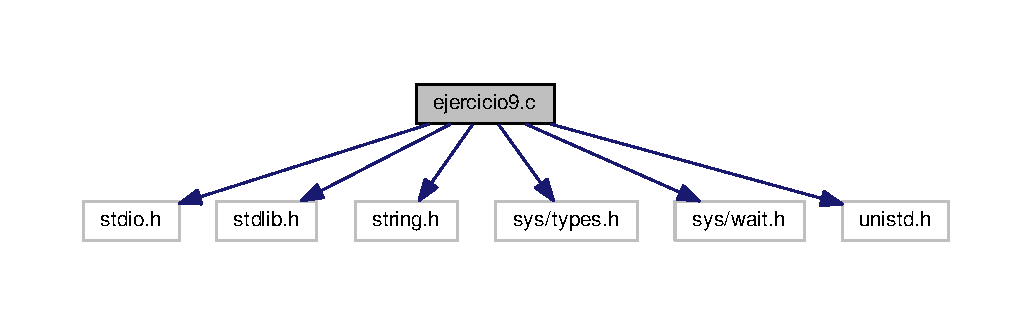
\includegraphics[width=350pt]{ejercicio9_8c__incl}
\end{center}
\end{figure}
\subsection*{\textquotesingle{}defines\textquotesingle{}}
\begin{DoxyCompactItemize}
\item 
\#define \hyperlink{ejercicio9_8c_acee2369f62e4a096d243dec3cd7d0b00}{N\+U\+M\+\_\+\+P\+R\+OC}~4
\end{DoxyCompactItemize}
\subsection*{Funciones}
\begin{DoxyCompactItemize}
\item 
int \hyperlink{ejercicio9_8c_a0ddf1224851353fc92bfbff6f499fa97}{main} (int argc, char $\ast$argv\mbox{[}$\,$\mbox{]})
\begin{DoxyCompactList}\small\item\em funcion en la que los hijos hacen las operaciones y el padre mostrara el mensaje \end{DoxyCompactList}\end{DoxyCompactItemize}


\subsection{Descripción detallada}
Implementa el ejercicio 9 de tuberias. 

\begin{DoxyAuthor}{Autor}
Andres Salas \href{mailto:andres.salas@estudiante.uam.es}{\tt andres.\+salas@estudiante.\+uam.\+es} 

Antonio Martin \href{mailto:antonio.martinmasuda@estudiante.uam.es}{\tt antonio.\+martinmasuda@estudiante.\+uam.\+es} 
\end{DoxyAuthor}
\begin{DoxyNote}{Nota}
Grupo 2202 
\end{DoxyNote}
\begin{DoxyVersion}{Versión}
1.\+0 
\end{DoxyVersion}
\begin{DoxyDate}{Fecha}
10/02/2017 
\end{DoxyDate}


\subsection{Documentación de los \textquotesingle{}defines\textquotesingle{}}
\index{ejercicio9.\+c@{ejercicio9.\+c}!N\+U\+M\+\_\+\+P\+R\+OC@{N\+U\+M\+\_\+\+P\+R\+OC}}
\index{N\+U\+M\+\_\+\+P\+R\+OC@{N\+U\+M\+\_\+\+P\+R\+OC}!ejercicio9.\+c@{ejercicio9.\+c}}
\subsubsection[{\texorpdfstring{N\+U\+M\+\_\+\+P\+R\+OC}{NUM_PROC}}]{\setlength{\rightskip}{0pt plus 5cm}\#define N\+U\+M\+\_\+\+P\+R\+OC~4}\hypertarget{ejercicio9_8c_acee2369f62e4a096d243dec3cd7d0b00}{}\label{ejercicio9_8c_acee2369f62e4a096d243dec3cd7d0b00}
Numero de hijos a crear 

\subsection{Documentación de las funciones}
\index{ejercicio9.\+c@{ejercicio9.\+c}!main@{main}}
\index{main@{main}!ejercicio9.\+c@{ejercicio9.\+c}}
\subsubsection[{\texorpdfstring{main(int argc, char $\ast$argv[])}{main(int argc, char *argv[])}}]{\setlength{\rightskip}{0pt plus 5cm}int main (
\begin{DoxyParamCaption}
\item[{int}]{argc, }
\item[{char $\ast$}]{argv\mbox{[}$\,$\mbox{]}}
\end{DoxyParamCaption}
)}\hypertarget{ejercicio9_8c_a0ddf1224851353fc92bfbff6f499fa97}{}\label{ejercicio9_8c_a0ddf1224851353fc92bfbff6f499fa97}


funcion en la que los hijos hacen las operaciones y el padre mostrara el mensaje 

\begin{DoxyReturn}{Devuelve}
int\+: valor de exito o fracaso 
\end{DoxyReturn}

%--- End generated contents ---

% Index
\backmatter
\newpage
\phantomsection
\clearemptydoublepage
\addcontentsline{toc}{chapter}{Índice}
\printindex

\end{document}
